\documentclass{article}

\usepackage{graphicx}
\usepackage{tikz}
\usepackage{tikzsymbols}
\usetikzlibrary{calc,patterns,shapes.geometric}
\pagestyle{empty}
\usepackage[margin=0pt]{geometry}
\geometry{papersize={14in,12in}}

\def\centerarc[#1](#2)(#3:#4:#5){\draw[#1] ($(#2)+({#5*cos(#3)},{#5*sin(#3)})$) arc (#3:#4:#5);}

\begin{document}
	\begin{figure}
		\centering
		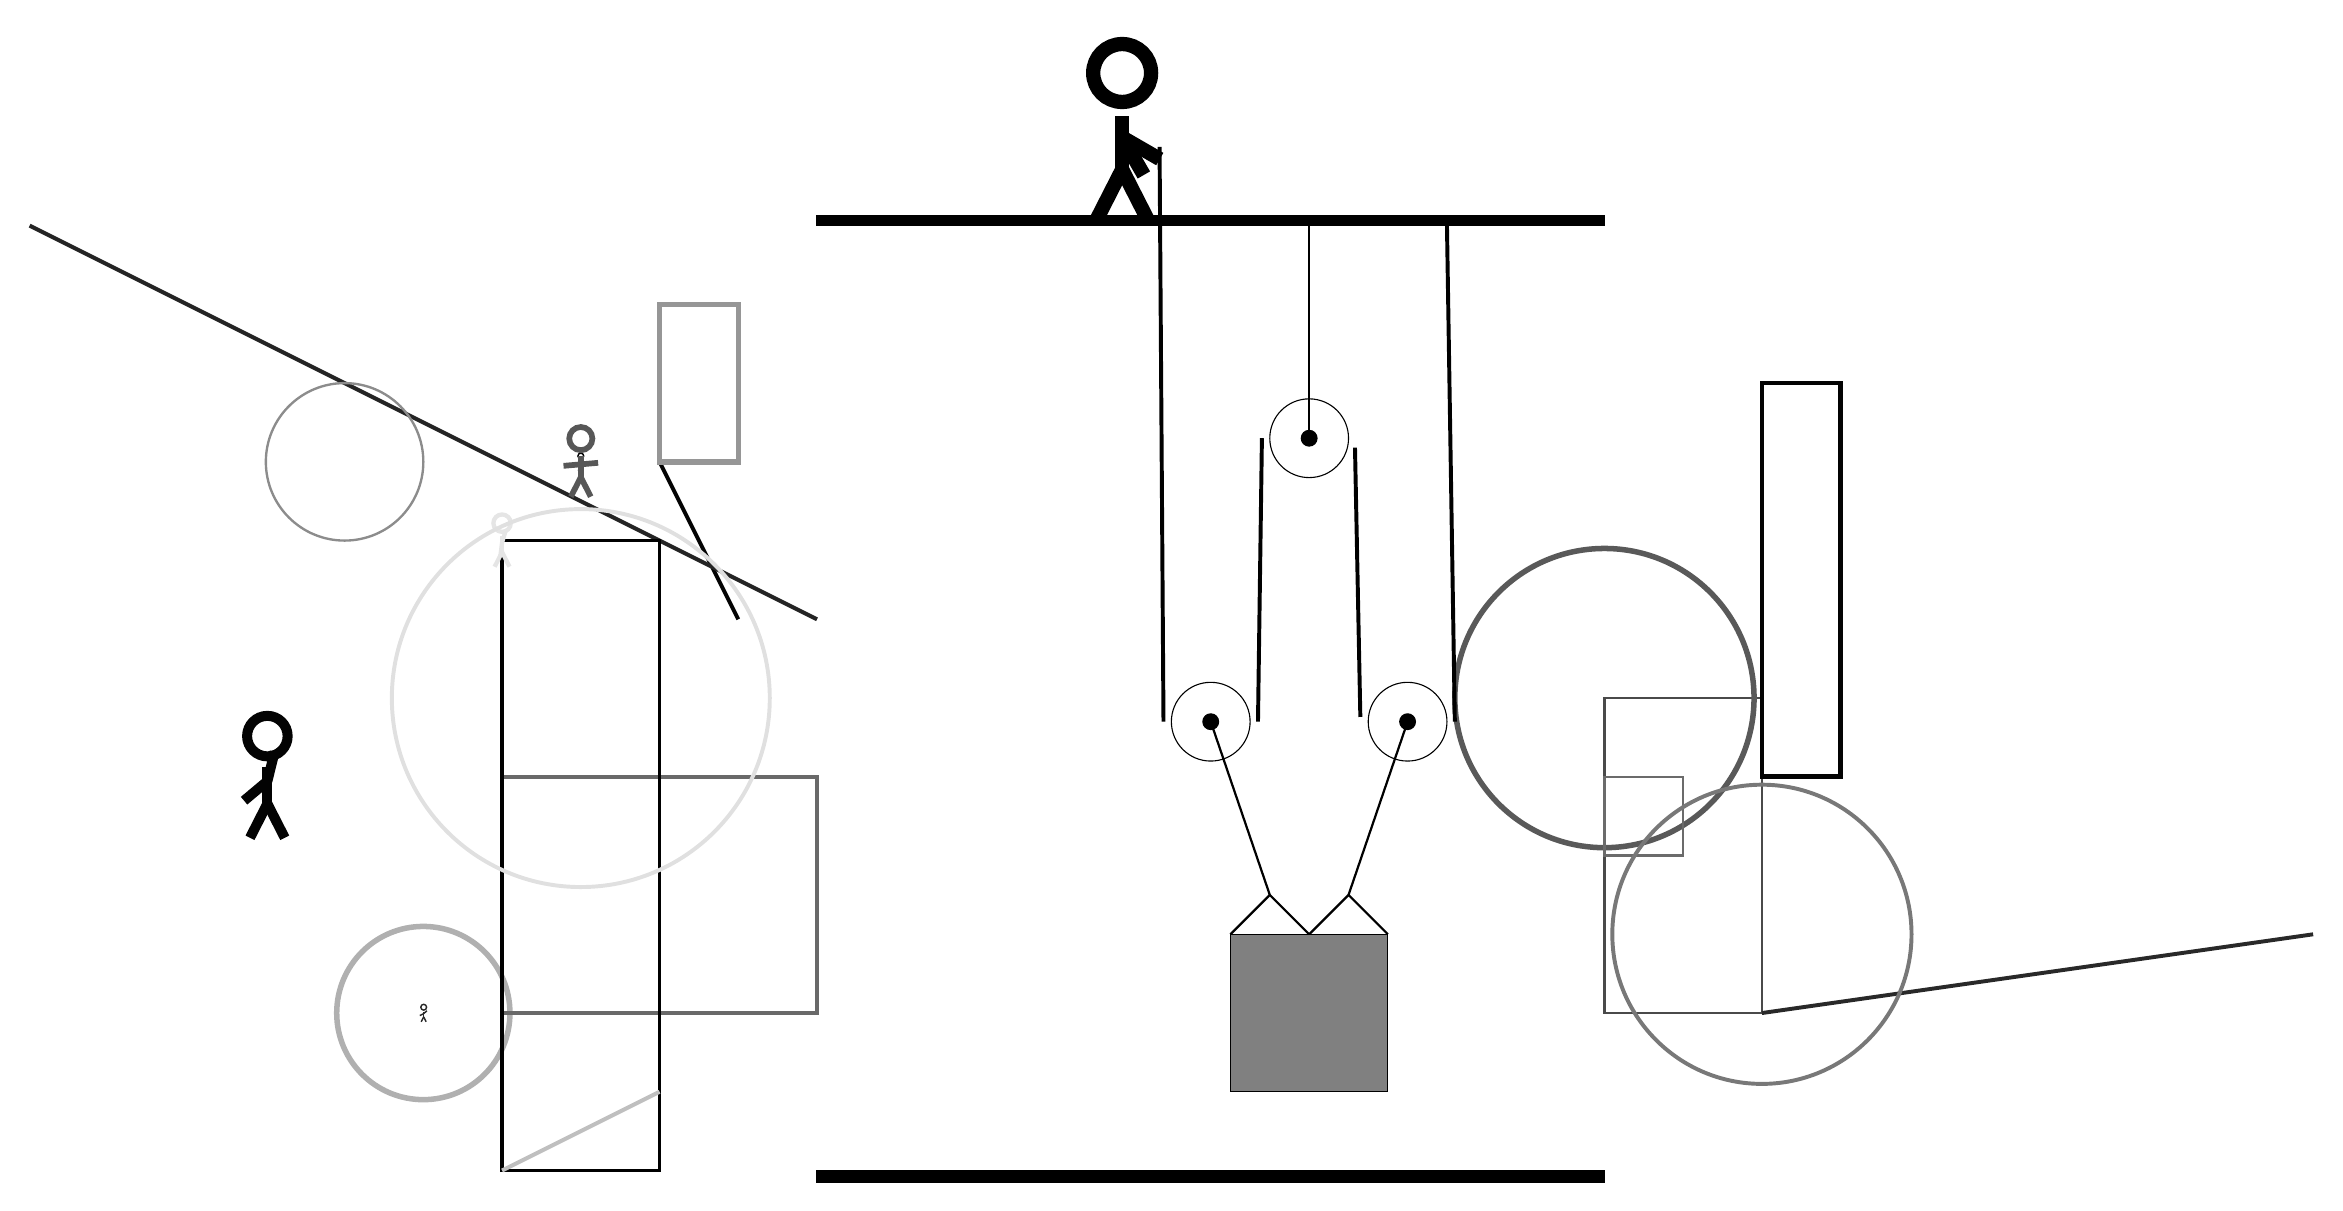
\begin{tikzpicture}
			%%%%% START %%%%%
			
			\draw[fill=black] (-4, 9) rectangle (6, 9.125);
			
			\draw (1, 2.7) circle (0.5);
			\draw[fill=black] (1, 2.7) circle (0.1);
			
			\draw (2.25, 6.3) circle (0.5);
			\draw[fill=black] (2.25, 6.3) circle (0.1);
			\draw[thick] (2.25, 6.3) -- (2.25, 9);
			
			\draw[line width=0.3mm, color=black!71] (8, 3) rectangle (6, -1);
			
			\draw[line width=0.5mm, color=black!99](-6, 6) -- (-5, 4);
			\draw [line width=0.7mm, color=black!65](6, 3) circle (1.9);
			\draw[line width=0.5mm, color=black!86](-4, 4) -- (-14, 9);
			
			\draw [line width=0.7mm, color=black!31](-9, -1) circle (1.1);
			
			\draw[line width=0.5mm, color=black!59] (-4, 2) rectangle (-8, -1);
			\node[line width=0.6mm, color=black!99] at (-11, 2) {\Strichmaxerl[7][40][76]};
			
			\node[line width=0.3mm, color=black!99] at (-7, 6) {\Strichmaxerl[1][80][56]};
			\draw[line width=0.4mm, color=black!100] (-6, -3) rectangle (-8, 5);
			
			\draw[line width=0.3mm, color=black!58] (6, 1) rectangle (7, 2);
			
			\draw[line width=0.5mm, color=black!25](-6, -2) -- (-8, -3);
			\node[line width=0.5mm, color=black!10] at (-8, 5) {\Strichmaxerl[3][83][73]};
			\draw[line width=0.6mm, color=black!99] (8, 2) rectangle (9, 7);
			\draw[line width=0.5mm, color=black!84](8, -1) -- (15, 0);
			\node[line width=0.5mm, color=black!66] at (-7, 6) {\Strichmaxerl[4][5][5]};
			\draw [line width=0.5mm, color=black!12](-7, 3) circle (2.4);
			\draw [line width=0.3mm, color=black!45](-10, 6) circle (1.0);
			\draw [line width=0.5mm, color=black!53](8, 0) circle (1.9);
			\draw[line width=0.4mm, color=black!81] (-6, 1) rectangle (-6, 1);
			\draw[line width=0.7mm, color=black!41] (-6, 8) rectangle (-5, 6);
			\node[line width=0.5mm, color=black!84] at (-9, -1) {\Strichmaxerl[1][26][42]};
			
			
			\draw (3.5, 2.7) circle (0.5);
			\draw[fill=black] (3.5, 2.7) circle (0.1);
			
			\draw[thick] (3.5, 2.7) -- (2.75, 0.5);
			\draw[thick] (1, 2.7) -- (1.75, 0.5);
			\draw[thick]  (1.25, 0) -- (1.75, 0.5) -- (2.25, 0);
			\draw[thick]  (2.25, 0) -- (2.75, 0.5) -- (3.25, 0);
			\draw[fill=black!50] (1.25, 0) rectangle (3.25, -2);
			
			\draw[line width=0.5mm] (0.35, 10) --  (0.4, 2.7);
			\centerarc[line width=0.5mm](1, 2.7)(180:360:0.6);
			\draw[line width=0.5mm] (1.6, 2.7) -- (1.65, 6.3);
			\centerarc[line width=0.5mm](2.25, 6.3)(-20:180:0.6);
			\draw[line width=0.5mm](2.832, 6.18) -- (2.9, 2.76);
			\centerarc[line width=0.5mm](3.5, 2.7)(160:360:0.6);
			\draw[line width=0.5mm](4.1, 2.7) -- (4.0, 9);
			
			\node at (-0.07, 10.2) {\Strichmaxerl[10][120][-30]};
			
			\draw[fill=black] (-4, -3) rectangle (6, -3.15);
			
			%%%%% END %%%%%
		\end{tikzpicture}
	\end{figure}	
\end{document}